% Chapter Template

\chapter{Introduction} % Main chapter title

\label{Chapter 1} % Change X to a consecutive number; for referencing this chapter elsewhere, use \ref{ChapterX}

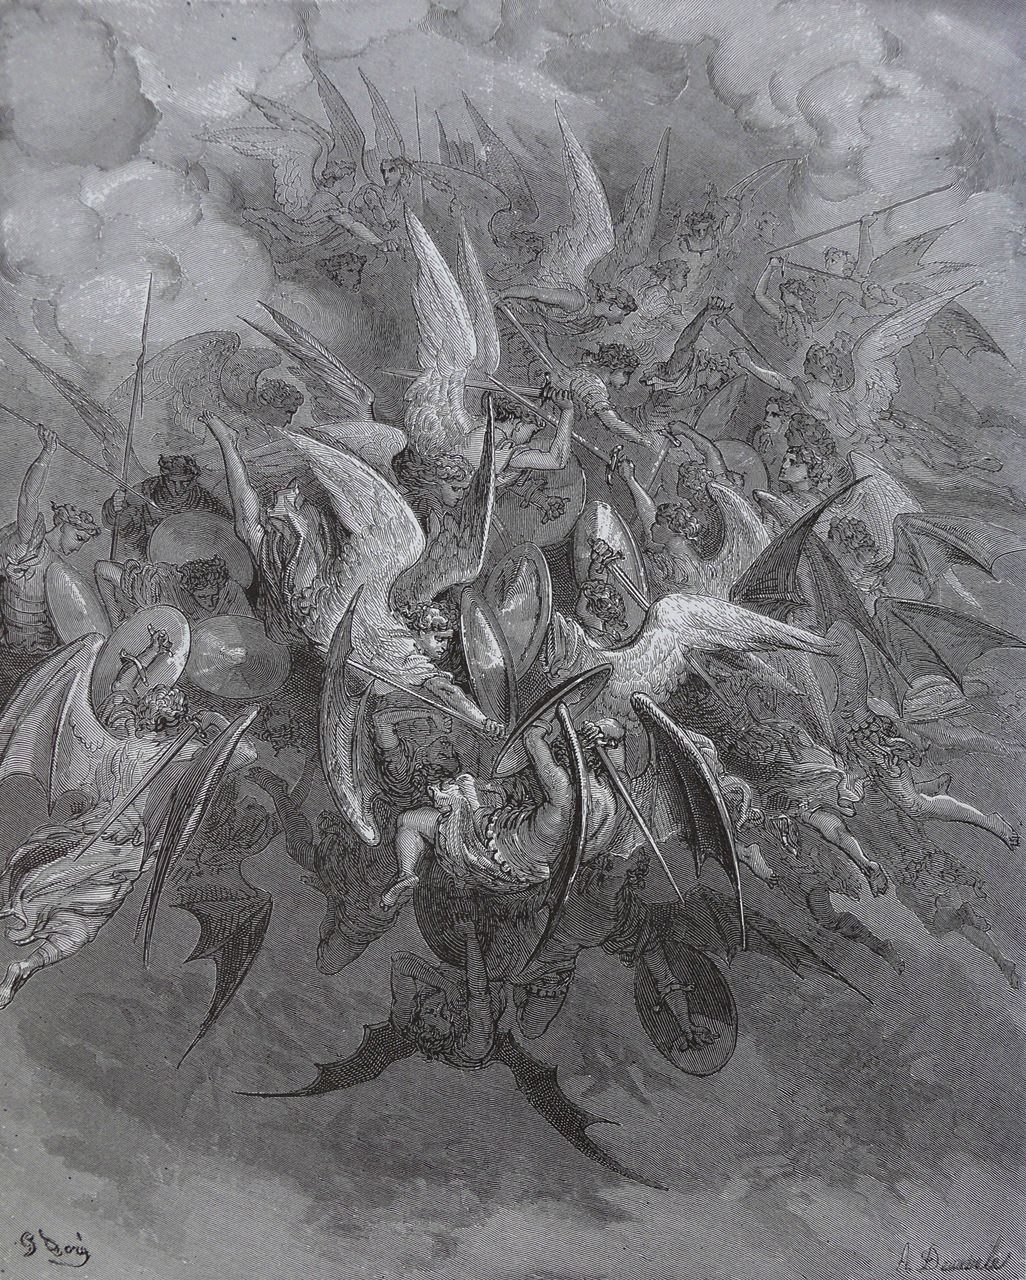
\includegraphics[width=\linewidth,trim={0 9cm 0 10cm},clip]{Paradise_Lost_24}

\section{Paradise Lost}

\label{Ch1 Sec1}

The earliest epochs of the digital era were based on a sense of control and security:  A computational device could be
created, and could be expected to behave as expected, and not to be subverted at a distance by invisible hands.
This began with the first computers that were the size of a small building, and continued until the advent of personal
computers that were capable of easy exchange of data between them, initially by floppy disk, by modem or
other forms of networking \cite{chen2004evolution}. 
Essentially, whenever a means of communications was established between computers, worms, virii and other
pathological software soon followed.   The pathological software was initially simple in nature, and
could be easily detected and removed, and into the 1990s it was not uncommon to be able to obtain anti-virus
software that could detect and remove all extant pathological software from a system.
Figure \ref{fig:nortonad} shows an example advertisement from 1991, which explains that if users suspect
the existence of a new virus, they can call a ``24-hour virus newsline'', betraying how relatively
sedate the development and spread of computer virii was at that time.

\begin{figure}
  \label{fig:nortonad}
  \centering
  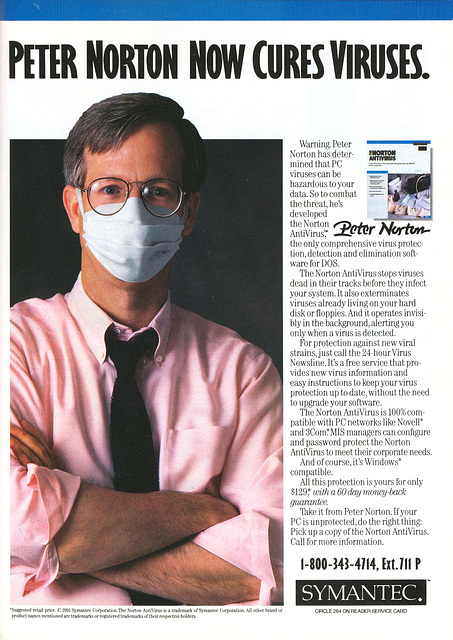
\includegraphics[width=\linewidth]{NortonAntiVirus-Advertisement}
  \caption{Early advertisement for Norton Anti-Virus for DOS. New viruses spread slowly at the time, as they could
    only be spread by floppy disk. As a result, users could be reasonably directed to call a telephone number if they
    suspected that they had a new virus on their computer. Source: \url{http://www.ipernity.com/doc/78280/6670939}.
    }
\end{figure}

The advent of ubuiquitous internet access marked a dramatic shift:  Where as previously viruses were mostly reliant on the
movement of physical artefacts, such as floppy disks, the internet allowed for the infection of systems anywhere in the
world, without coming into physical contact.
That is, it introduced a new and highly effective transmission mode, that was all the more insidious in that in the floppy-era
you could determine whether your computer might be at risk, based on whether it had been in contact through the insertion of
a floppy disk.
This allowed for individuals to effectively manage the sanitation of their computers in a rational and understandable manner.
The Internet allowed for invisible infection at a distance, a problem which persists to the present day, and which has created
the conditions for the wide range of malware, viruses, trojan software, ransomware, rootkits, backdoors and other pathological
software to develop and spread.

This evolution of the pathogenic material to take advantage of the available modes of delivery is directly mirrored in the
world of biology \cite{antonovics2017evolution}.
Indeed, what we see with computers now, is that the defences against these infectious threats have come to resemble the
immune system of complex animals: A variety of intrinsic protections, heuristic measures and the development of immunity only
after infection have become accepted norms for computer security.
However, this is a dangerous situation, just as animals are made sick or die or are subverted by biological pathogens, e.g., Figure \ref{fig:antzombies}), the
compromise of our digital systems has significant effects for individuals and society.  And just as it is impossible to quickly
appraise whether an animal is free of all disease, it has become impossible to determine authoritatively whether a computer
is free of all digital pathogens.

\begin{figure}
  \label{fig:antzombies}
  \centering
  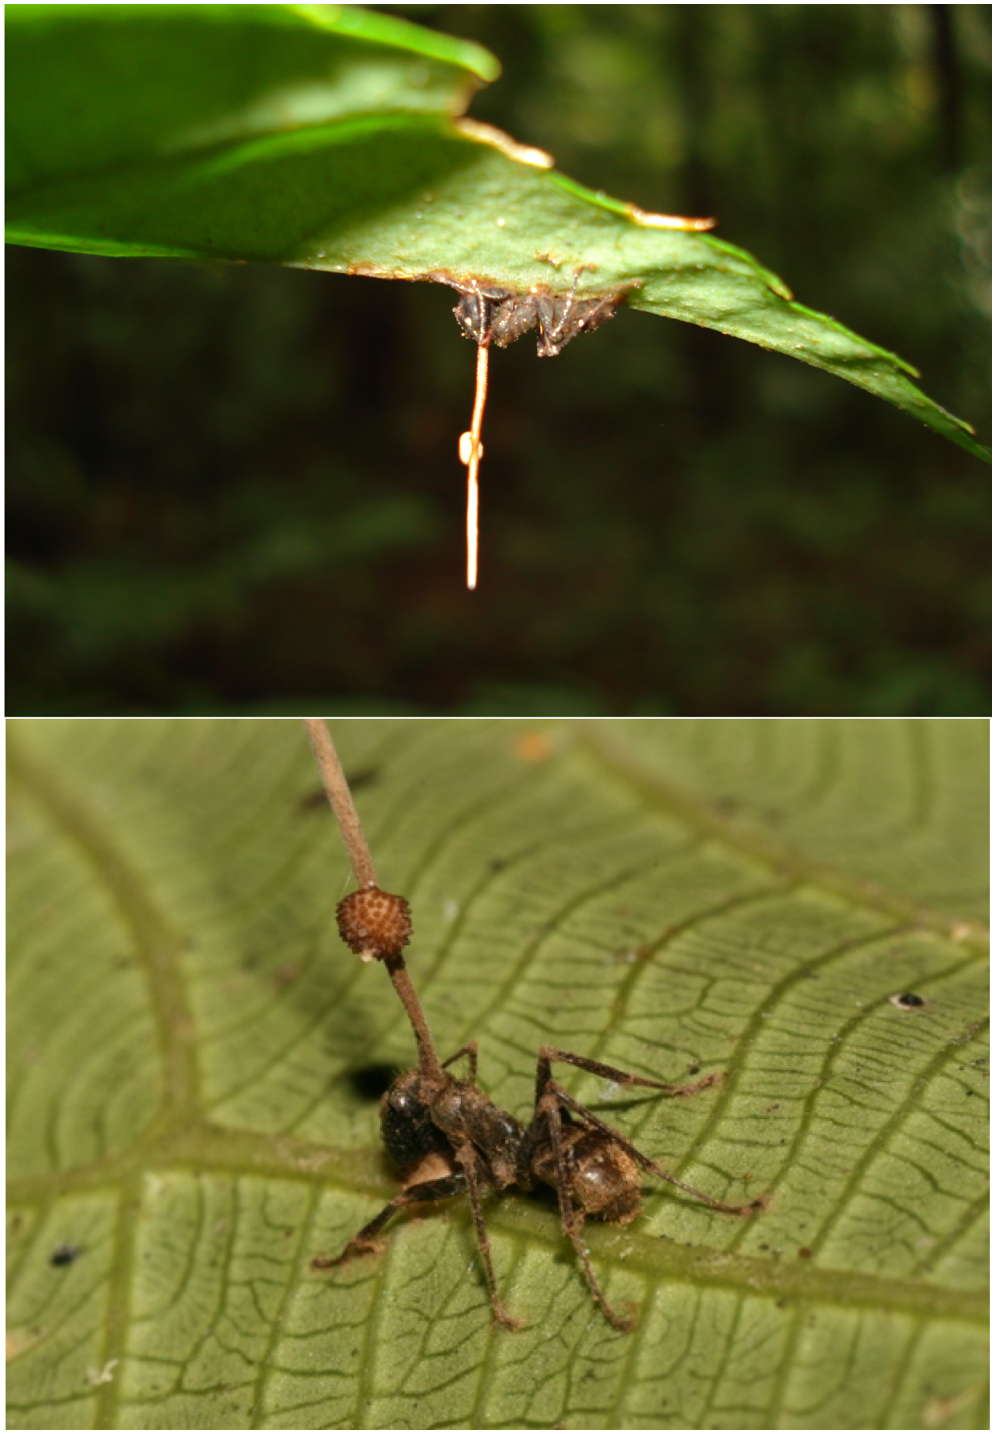
\includegraphics[width=0.8\linewidth]{Ophiocordyceps_unilateralis}
  \caption{
    {\em Ophiocordyceps unilateralis} is perhaps better known as the ``zombie ant fungus''.  When it infects an ant,
    it modifies the ant's behaviour, so that it leaves its ground-based nest-mates, climbs a tree and finds a leaf,
    and bites into the underside of the leaf so that it hangs upside down. Several days later the fungus emerges from
    the head of the ant in a fruiting body that showers its nest-mates with spores, thus spreading quickly through
    entire colonies.  Source: 
    \url{https://upload.wikimedia.org/wikipedia/commons/8/85/Ophiocordyceps_unilateralis.png}
  }
    
\end{figure}

\todo{Add HIV/BADBIOS and IME/auto-immune analogies here if you wish}

Were this not depressing enough, the problem is complicated by the fact that computers have, like biological organisms,
become so complex, that it is impossible to construct them in such a way that they can effectively resist being subverted.
The interactions in modern software are now so rich -- like the interactions of proteins, genes and other elements that make up
the control machinery of living cells -- that it is impossible to fully understand them in all but the most trivial of circumstances.

This problem has been compounded by Moore's Law \todo{cite}, which has made it cheaper to create ever more complex computers, and
by human psychology which have created an emphasis on the number of features or functions of a given piece of software, rather than
on its correctness and security.  Thus software has exploded in size from kilo-bytes in the early 1980s to tens of giga-bytes in
the current era. That is, software is now often millions of times larger and more complex than it once was, to the poinnt where
verification of correctness has become effectively impossible.

As bad as this situation is for software, it is even worse when hardware systems are considered, and the central processing units
(CPUs) of computers in particular.  CPUs have also grown in complexity from thousands of transistors to tens of billions of transistors
over the same time period.  However, unlike a defect in software, a defect in a CPU cannot necessarily be corrected without physical
replacement.

The fact that the Spectre and MELTDOWN vulnerabilities existed in CPUs for almost 20 years before being discovered \todo{cite}
is strong evidence that we have long since passed the point where even a well-resourced company like Intel or AMD can ensure
the correct operation of a CPU.  If these companies with many thousands of verification engineers cannot achieve it,
what hope do individuals and small organisations have for verifying the correct operation of their computing devices?

What is clear is that the problem is one of complexity: A single transistor can be easily verified. The simple early CPU designs
like the 6502, that consisted of only a few thousand transistors can also be easily verified.  But modern complex CPU designs cannot.
There must exist somewhere a tipping point where verification ceases to be realistic for a determined user.
Beyond that point security is merely a hopeful dream, because we can no longer prove correctness and immunity to the challenges
that it might face, just as avoiding the common cold is also no more than a hopeful dream, and certainly nothing that can
be guaranteed if we are to remain in communications with the outside world.

We are therefore forced to accept the unpalatable truth that we are no more sovereign over our computing devices than our bodies
are over the biological world that surrounds us: We have been cast from the Eden of security for eating the forbidden fruit of
ever increasing complexity and functionality.

The question is whether we can go back, to create computing devices that are sufficiently simple as to be securable, and yet
remain sufficiently useful in practice.  This is the motivating question for this thesis.

\section{Research Questions}

\label{Ch1 Sec2}

What are the missing or non-functional sub-systems that the MEGA65 requires to be implemented?\\*
Which will be answered in the form of a survey of the current sub-systems of the MEGA65, and a survey of the sub-systems required to create a functional prototype.\\
\\
How can these sub-systems be implemented?\\
Which will be answered by the creation of plans for the implementing of the missing or incomplete sub-systems.\\
\\
How can the simplicity, understandability and hence, the security of these sub-systems be maximised?\\
Which will be answered by considering each sub-system, qualitatively appraising its simplicity, understandability and security, and where appropriate, making well researched recommendations for refining those components to improve one or more of these axes, and time permitting, acting on those recommendations.\\
\\
How can the complete MEGA65 architecture be physically prototyped on the bench?\\
Which will be answered by examination of the current partial bench prototype and comparing it with the sub-systems identified through the other research questions, and designing and realising a complete bench prototype.
This will occur through coordination with Mr. Lachlan McDonald, who is undertaking the designing of the PCB for the MEGA65 smart-phone device.\\
\\
How can the secure compartmentalisation's architecture planned for the MEGA65 be realised?\\
Which will be answered by considering this architecture and the current state of the MEGA65 system to derive and execute a method for implementing a secure compartmentalisation architecture.\\
\\
Overall the success of the project will be measured against the creation of a functioning bench prototype device that, through the architecture, implements the secure and understandable compartmentalisation of hardware to the point of demonstrability.

%----------------------------------------------------------------------------------------
%	SECTION 3
%----------------------------------------------------------------------------------------

\section{Thesis Layout}

\label{Ch1 Sec3}

Following this chapter, "Chapter \ref{Chapter 1} : Introduction", is the chapter, "Chapter \ref{Chapter 2} : Literature Review".
In which relevant background information regarding complexity and cyber security, mobile devices, isolative security and the MEGA65 project will be given.
After this, "Chapter \ref{Chapter 3} : Methods and Materials" will go on to describe how this project was undertaken and what tools were used.
This will be immediately followed by "Chapter \ref{Chapter 4} : Project Set-up".
In this chapter, details about the issues faced immediately after joining the project will be made clear.
Following this is "Chapter \ref{Chapter 5} : Matrix Mode Corrections", in this chapter the issues encountered with the matrix mode and their fixes will be made clear.
"Chapter \ref{Chapter 6} : Secure Compartmentalisation" will follow, in which an overview of how the secure containers in the phone were implemented will be given.
This will be followed by "Chapter \ref{Chapter 7} : Results and Discussion" where XXX will be talked about.
Finally, "Chapter \ref{Chapter 8} : Conclusion" will discuss the various details about the findings of this document, as well as the discuss the research questions outlined in section \ref{Ch1 Sec2 Sub3}. In addition to this, the future works for the secure compartment and matrix mode portions of the project will be outlined.

